%!TEX root = ../thesis.tex
%*******************************************************************************
%****************************** Second Chapter *********************************
%*******************************************************************************

\chapter{Simulation and Reconstruction}

The simulation of signal as well as background events is a critical part of the measurement
of the \ttbar cross section. The first step is the simulation of the result of the proton-proton 
collisions at a center of mass energy of $\sqrt{s} = 13 \; \TeV$. Then the decay and further interaction 
of the resulting particles is predicted. The final step is the simulation of the detector response.
Single events including all relevant particles and their kinematics are simulated.
The whole process is described in detail in Section \ref{sec:SimReco_Sim}.

In order to be analyzed, both the data and the simulation need to be reconstructed. The same algorithms are applied to ensure
that the simulation consistently models the data. 
The whole detector information is used to reconstruct particles and physics objects like electrons or jets.
The details can be found in Section \ref{sec:SimReco_Reco}. 


\section{Simulation}
\label{sec:SimReco_Sim}

The simulation of events involves multiple algorithms.
The scattering amplitude is calculated with a matrix element generator. These calculations rely on the factorisation of the impact of the proton substructure and the hard 
interactions of the partons. The proton substructure is given by a Parton Density Function (PDF) which gives the probability of a given parton to carry a certain momentum fraction 
at factorisation scale $\mu_F$. The hard interaction itself is calculated depending on the energy fraction of the two partons in the initial state at the so called renormalisation scale $\mu_R$.
For the simulation of the \ttbar signal process the scales are chosen as $\mu_R = \mu_F = \sqrt{m_t^2 + \pt^2}$.



The initial and final states are defined according to the process that is to be calculated and the scattering amplitude is computed at
a fixed order of QCD. In the context of this analysis multiple different matrix element generators are used depending on the respective process.



\section{Reconstruction}
\label{sec:SimReco_Reco}

Different particles deposit energy in different parts of the detector as illustrated in Figure \ref{fig:pflow}.
The tracks of charged particles are bent by the magnetic field, while neutral particles are unaffected.
Similarly only charged particles leave a signal in the tracker.
Electrons and photons deposit the main amount of their energy in the ECAL, whereas neutral and charged hadrons mainly deposit energy in the HCAL.
Muons are mainly detected by muon system in the outermost parts of the detector.
Phyics objects are reconstructed by combining this information from the basic elements of the detector using the Particle Flow algorithm \cite{Sirunyan:2017ulk}.

\begin{figure}[htbp!]
  \begin{center}
      \resizebox{0.80 \textwidth}{!}{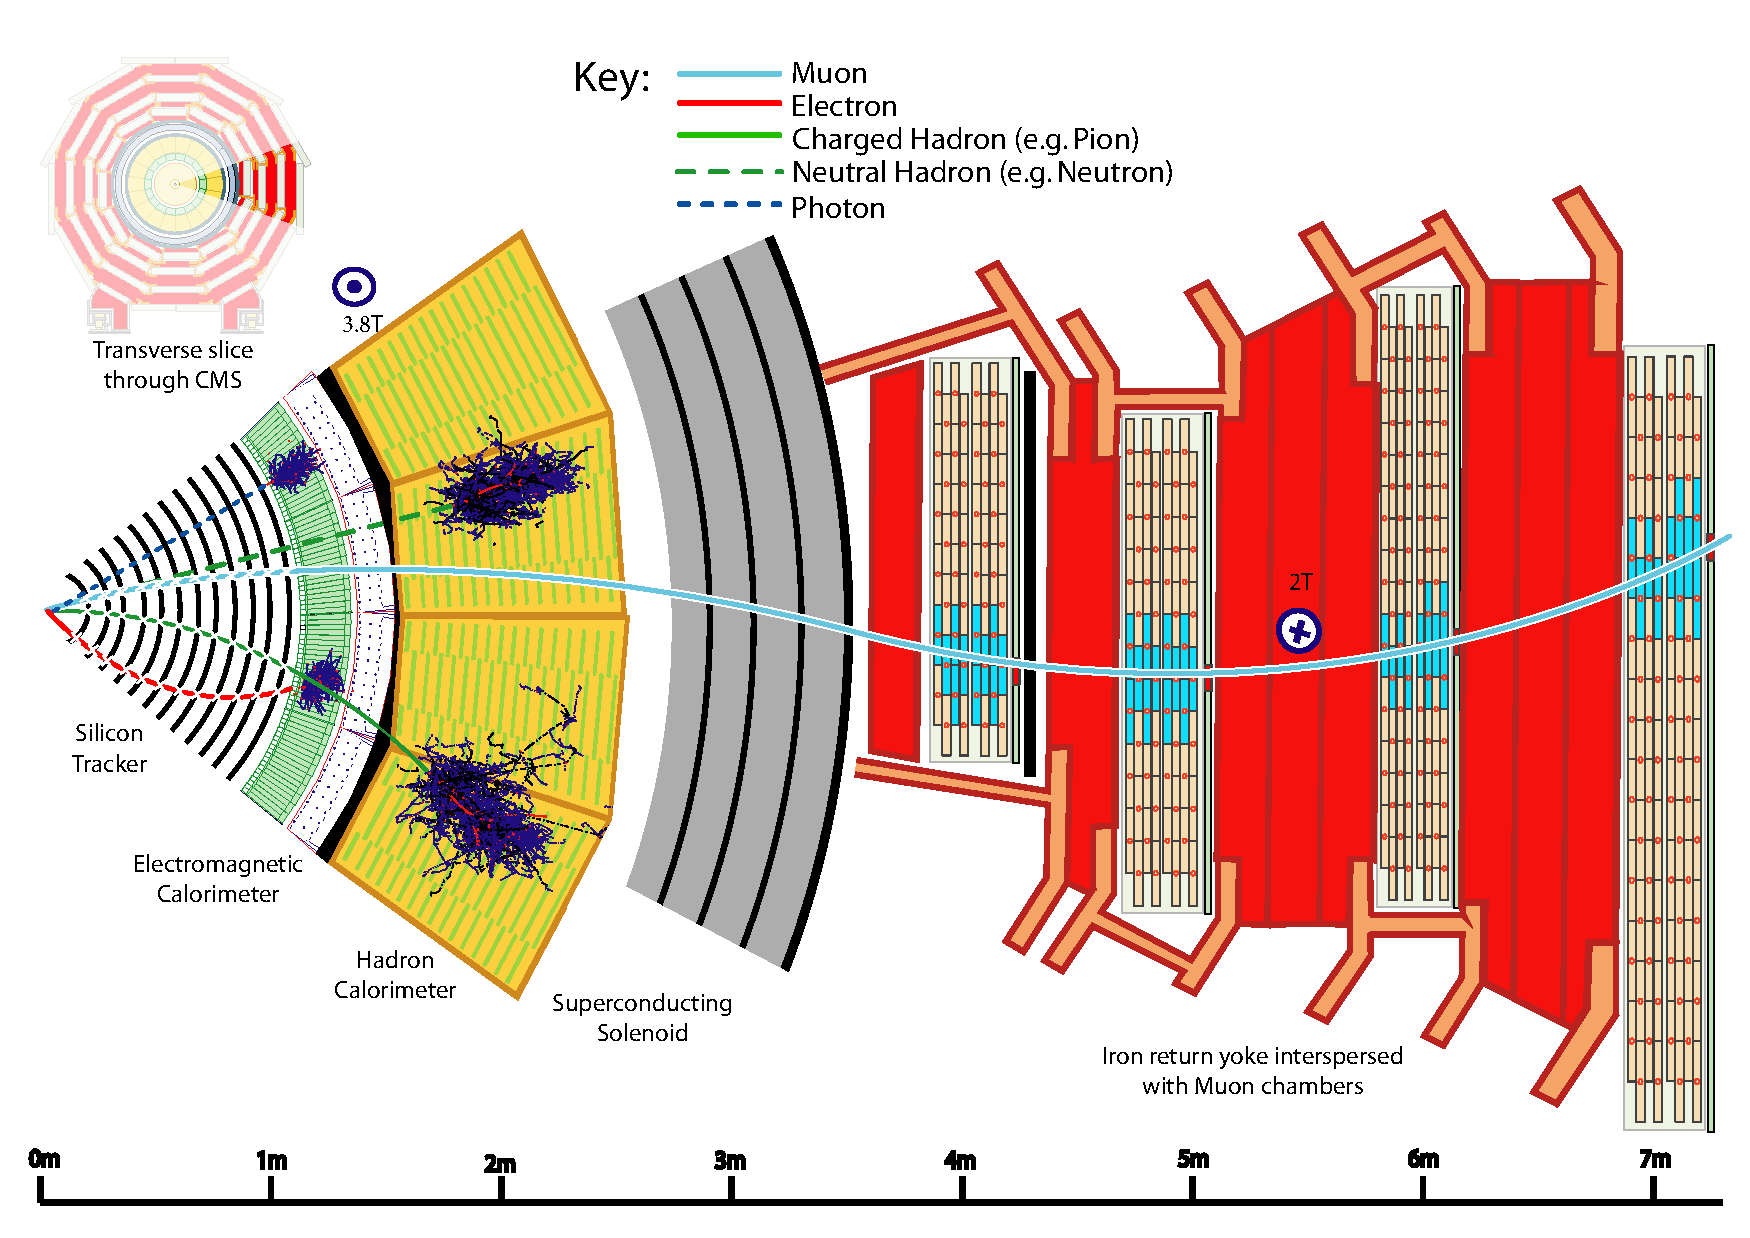
\includegraphics{SimReco/Figures/ParticleFlow.pdf}}
\caption{Illustration of the interaction of specific particles in a transverse slice of the CMS detector \cite{Sirunyan:2017ulk}.
  \label{fig:pflow}}
  \end{center}
\end{figure}

\subsection{Tracking and Vertex Reconstruction}

The aim of the tracking algorithm is to provide three properties of charged particles: The origin, the transverse momentum and the direction.
The track reconstruction itself is based on Kalman-Filtering \cite{Adam:934067} and consists of three steps starting with a seed of a few hits consistent with the trajectory of a charged particle.
The subsequent steps are the collection of hits from all tracker layers along the trajectory and the fitting to determin the aforementioned properties of the particle.
The tracking efficiency can be increased by repeating the track finding with different conditions.

The gain in efficiency through iterative tracking is presented in Figure \ref{fig:trackingEff} showing the efficiency and the misreconstruction rate for tracks depending on the \pt of the charged particle for 
multiple different tracking algorithms. The efficiency is determined in simulation where tracks are considered to be reconstructed correctly if they are associated to a simulated particle. Correspondingly 
misreconstructed tracks are not associated to a simulated particle. 
Including all iterations shows a the highest efficiency and a comparative mistag rate. In general the efficiency decreases dramatically for high \pt tracks, especially for tracks with $\pt > 100 \gev$.
Similarly, the misreconstruction rate increases with higher \pt, but the effect can be mitigated when the rest of the detector is taken into account.

\begin{figure}[htbp!]
  \begin{center}
      \resizebox{0.49 \textwidth}{!}{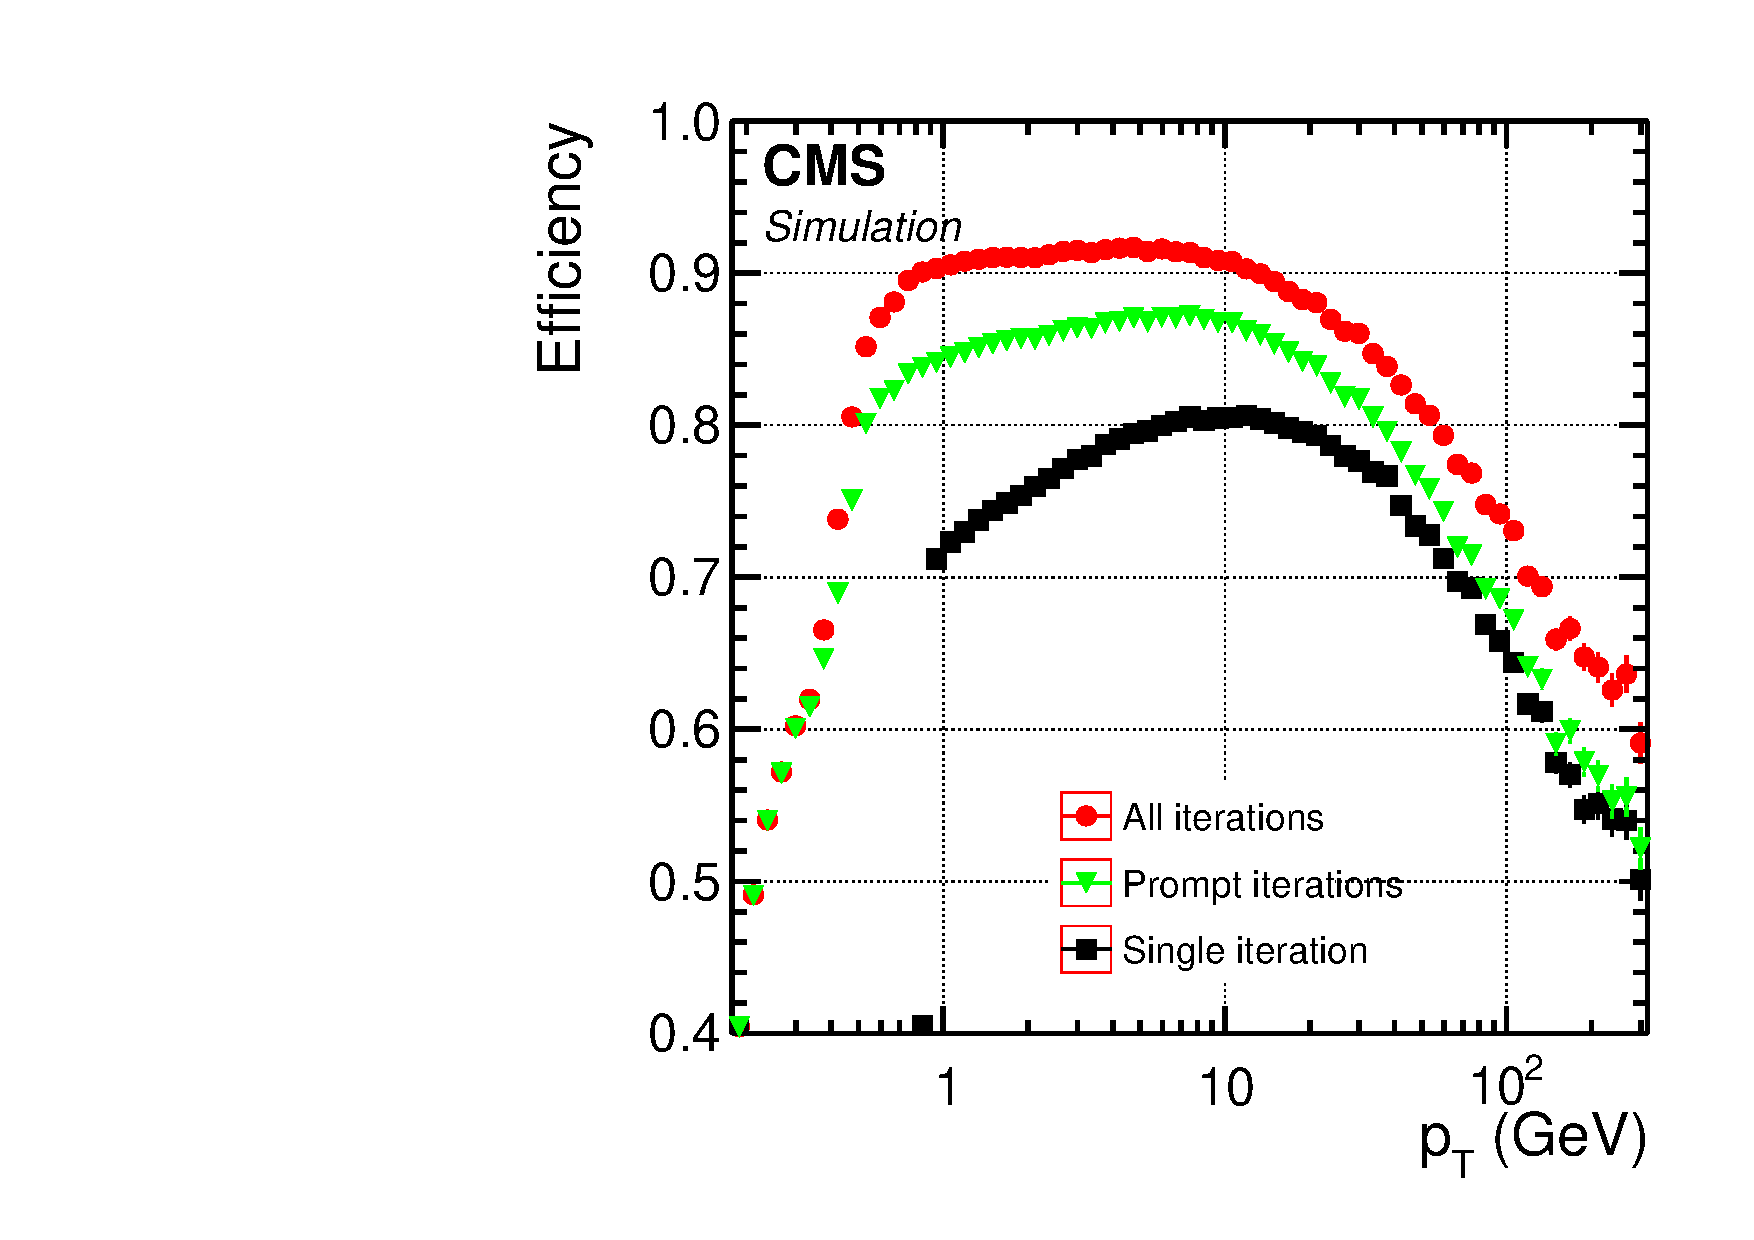
\includegraphics{SimReco/Figures/TrackingEff.pdf}}
      \resizebox{0.49 \textwidth}{!}{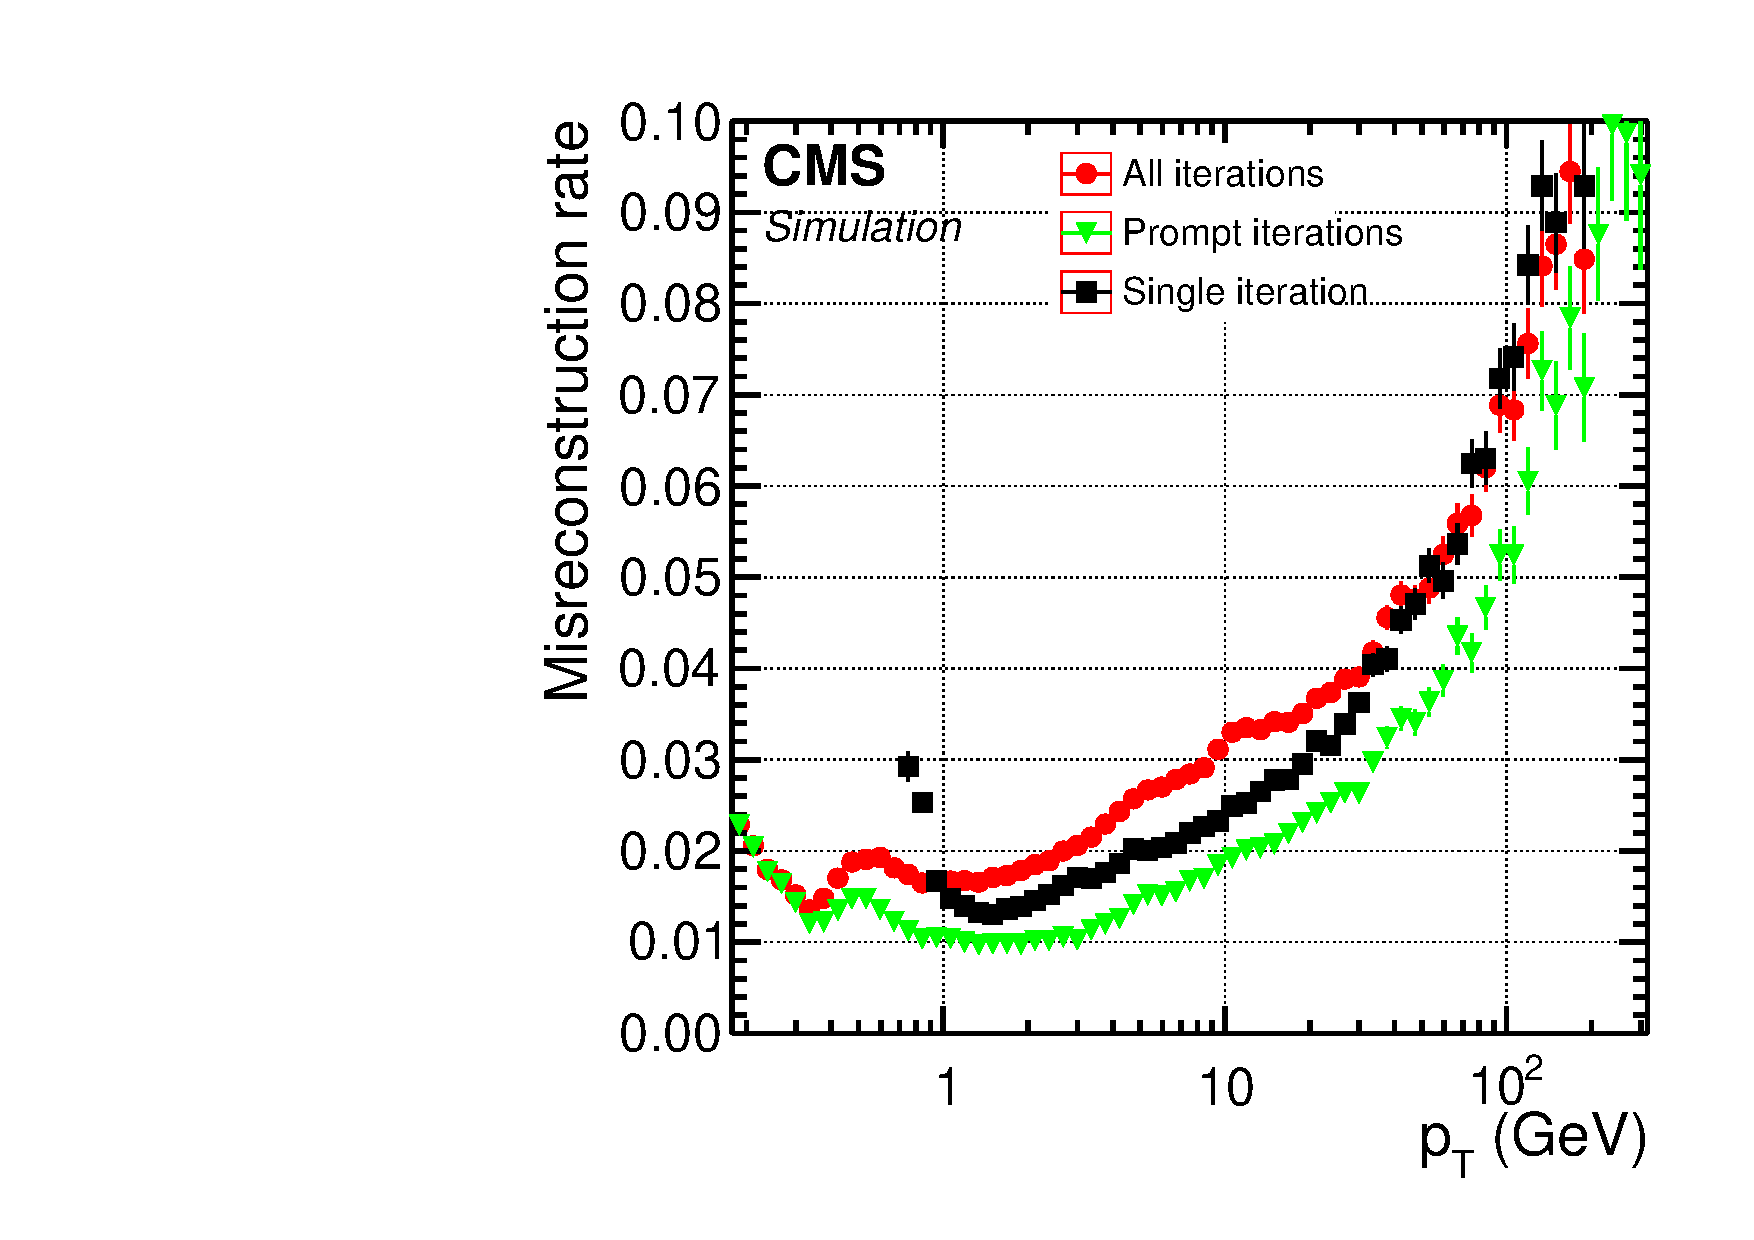
\includegraphics{SimReco/Figures/TrackingMis.pdf}}
\caption{Performance of the iterative tracking procedure\cite{Sirunyan:2017ulk}. The right plot shows the tracking efficiencies depending on the \pt of the charged particle for multiple different tracking approaches. 
         The left plot shows the rate to misreconstruct a track depending on the \pt of the charged particle for mutliple different tracking approaches. 
  \label{fig:trackingEff}}
  \end{center}
\end{figure}

The origins of the tracks along the beam axis are considered as primary vertices and sorted according to the \pt of the associated tracks.
The vertex with the highest \pt is considered to be connected to the hard interaction. 
Additional vertices are caused by additional proton proton collisions occuring in the same bunch crossing as the hard interaction.
This so called pile-up leads to an average of 16 primary vertices in the 2016 dataset. It is mitigated by removing the contribution from
the pile-up vertices from the reconstruction.

\subsection{Electron Reconstruction}

The reconstruction of electrons is based on the combination of information from the tracker and the calorimeters.
The ECAL cluster containing the energy deposited by the electron and the related bremstrahlung is needed for both photon and electron reconstruction.
The corresponding HCAL region is required to have a only 10 \% of the energy deposited in the ECAL to avoid contamination with hadrons.
In order to be identified as an electron a particle needs a cluster of ECAL energy to be associated with a track.
In case no track is found the particle is identified as a photon.

The association between ECAL cluster and track can be either seeded from the tracker or from the ECAL.
In order to increase the efficiency both approaches are combined \todo{add plots ?}.
Both the ECAL cluster and the track neeed to fullfill certain quality criteria applying to shower shape or track fitting.

Electrons are also required to be isolated: The energy deposited in a cone around an electron is required to be below 6 \% of the \pt of the electron.
The relative isolation is sensitive to contributions from pile-up. Contributions from charged particles that are not coming from the vertex of the hard collisions
are substracted from the isolation. The pile-up contributions from non-charged particles is harder to determin. It is estimated according to the general energy density
of the event and substracted from the isolation \todo{Plots ?}.

\subsection{Muon Reconstruction}

Muons leave tracks in both the tracker and the muon system. For a reconstructed global the track in the muon system has to be matched to a track in the tracker.
The tracks need to be compatible with each other when propagated to a common surface.
Further quality requirements are applied to the inner track in the tracker.

Similar to the electrons, the muns are also required to be isolated. The energy deposited in a cone around the muon (isolation) is required to be below 15 \% of the muon \pt.
This energy has to originate from charged particles coming from the primary vertex, neutral hadrons or photons. The impact of the pile-up on the neutral hadron and photon components
is estimated to be half of the contribution from charged pile-up and is substracted from the total isolation.

\todo{add some plots}


\subsection{Reconstruction of Jets and Identification of b-Jets}

Jets are clustered from the individual particles reconstructed from the particle flow algorithm \cite{CMS-PAS-JME-16-003}.
The clustering uses the anti-\kt algorithm \cite{Cacciari:2008gp} as implemented in \FASTJET \cite{Cacciari:2011ma} with a distance parameter of $R = 0.4$.
The impact of pile-iup is reduced by removing charged hadrons not originating from the primary vertex from the particles that are clustered \cite{CMS-PAS-JME-14-001}.
Neutral particles originating from pile-up are taken into account by correcting the jet 4-momenta for each event based on the jet area \cite{1126-6708-2008-04-005,CACCIARI2008119}.

The large lifetime of the B Hadron leads to a decay that is often displaced from the original interaction.
These secondary vertices together with the displaced tracks and the properties of the jet itself are combined in the CSVv2 algorithm to identify jets originating from a b quark \cite{BTV16002}.
Sensitive variables are combined into a neural network which is trained against both jets originating from light jets as well as jets originating from c quarks.
The result is a single value (discriminator) with the cut chosen according to the desired efficiency and background rejection.